\documentclass[aspectratio=169]{beamer}
\usetheme{Boadilla}
%\usetheme{Warsaw}
%\setbeamercovered{transparent}
\beamertemplatetransparentcoveredhigh
\usepackage[portuges]{babel}
\usepackage[utf8]{inputenc}
\usepackage{lmodern}
\usepackage[T1]{fontenc}
\usepackage[portuguese, linesnumbered, vlined, titlenumbered, ruled]{algorithm2e}
\SetKwRepeat{Registro}{registro \{}{\}}%
\usepackage{hyperref} 

\usepackage{xcolor}

\definecolor{codegreen}{rgb}{0,0.6,0}
\definecolor{codegray}{rgb}{0.5,0.5,0.5}
\definecolor{codepurple}{rgb}{0.58,0,0.82}
\definecolor{backcolour}{rgb}{0.95,0.95,0.92}

\usepackage{listings}
\lstdefinestyle{CStyle}{
    language=C++,
    backgroundcolor=\color{backcolour},   
    commentstyle=\color{codegreen},
    keywordstyle=\color{magenta},
    numberstyle=\tiny\color{codegray},
    stringstyle=\color{codepurple},
    basicstyle=\ttfamily\footnotesize,
    breakatwhitespace=false,         
    breaklines=true,                 
    keepspaces=true,                 
    numbers=left,       
    numbersep=5pt,                  
    showspaces=false,                
    showstringspaces=false,
    showtabs=false,                  
    tabsize=2,
}
% Macro que faz com que a numeracao de diferentes algoritmos continue de onde parou
\newcommand{\rememberlines}{\xdef\rememberedlines{\number\value{AlgoLine}}}
\newcommand{\resumenumbering}{\setcounter{AlgoLine}{\rememberedlines}}

\title[Aula Prática - Árvores AVL]{Algoritmos e Estrutura de Dados}
\subtitle{Árvores AVL}
\author[Frederico Santos de Oliveira]{prof. Frederico Santos de Oliveira}
\institute[UFMT]{Universidade Federal de Mato Grosso\\ Faculdade de Engenharia}
\date{}


\begin{document}

%%%%%%%%%%%%%%%%%%%%%%%%%%%%%%%%%%%%%%%%%%%%%%%%%%%%%%%%%%%%%%%%%%%%%%%%%%%%%%%%%%%%%%%%%%%%%%%%%%%%%%%%%

\begin{frame}[plain]
  \titlepage
\end{frame}

%%%%%%%%%%%%%%%%%%%%%%%%%%%%%%%%%%%%%%%%%%%%%%%%%%%%%%%%%%%%%%%%%%%%%%%%%%%%%%%%%%%%%%%%%%%%%%%%%%%%%%%%%
%\section*{Roteiro}

\begin{frame}
  \frametitle{Agenda}
  \tableofcontents
\end{frame}

%%%%%%%%%%%%%%%%%%%%%%%%%%%%%%%%%%%%%%%%%%%%%%%%%%%%%%%%%%%%%%%%%%%%%%%%%%%%%%%%%%%%%%%%%%%%%%%%%%%%%%%%%

\begin{frame}
\frametitle{Exercício}
Vamos implementar a estrutura de dados Árvore AVL.
\end{frame}

%%%%%%%%%%%%%%%%%%%%%%%%%%%%%%%%%%%%%%%%%%%%%%%%%%%%%%%%%%%%%%%%%%%%%%%%%%%%%%%%%%%%%%%%%%%%%%%%%%%%%%%%%
\section{Estrutura Nodo}
%%%%%%%%%%%%%%%%%%%%%%%%%%%%%%%%%%%%%%%%%%%%%%%%%%%%%%%%%%%%%%%%%%%%%%%%%%%%%%%%%%%%%%%%%%%%%%%%%%%%%%%%%

\begin{frame}{Árvore AVL}{Implementação}
Uma Árvore AVL é formada pela estrutura {\bf nodo}, que contém três campos:
\begin{itemize}
 \item Um ponteiro {\bf esq}, que indica o filho da esquerda daquele nodo.
 \item Um ponteiro {\bf dir}, que indica o filho da direita daquele nodo.
 \item Um campo {\bf item} do tipo {\bf int}, que é o tipo de dado a ser armazenado no nodo da árvore.
\end{itemize}
\begin{figure}[!h]
  \centering
  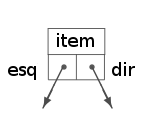
\includegraphics[width=70pt]{imagens/nodo.png}
  \label{fig_nodo}
\end{figure}
\end{frame}

%%%%%%%%%%%%%%%%%%%%%%%%%%%%%%%%%%%%%%%%%%%%%%%%%%%%%%%%%%%%%%%%%%%%%%%%%%%%%%%%%%%%%%%%%%%%%%%%%%%%%%%%%

\begin{frame}[fragile]{Árvore AVL}{Estrutura Nodo}
Segue o pseudo-código referente à estrutura nodo:
\begin{algorithm}[H]
\caption{Nodo} 
\label{Nodo}
\Inicio{
 \Registro{Nodo}{
    Inteiro: item; \\
    Inteiro: altura; \\
    Ponteiro Nodo: esq; \\
    Ponteiro Nodo: dir; 
  }
}
\end{algorithm} 
\end{frame}

%%%%%%%%%%%%%%%%%%%%%%%%%%%%%%%%%%%%%%%%%%%%%%%%%%%%%%%%%%%%%%%%%%%%%%%%%%%%%%%%%%%%%%%%%%%%%%%%%%%%%

\begin{frame}[fragile]{Árvore AVL}{Estrutura Nodo}
Na linguagem C, a implementação fica conforme o código a seguir:
\begin{lstlisting}[style=CStyle]
typedef struct nodo_t
{
    int item;
    int altura;
    struct nodo_t *esq;
    struct nodo_t *dir;
} nodo;
\end{lstlisting}  
\end{frame}


%%%%%%%%%%%%%%%%%%%%%%%%%%%%%%%%%%%%%%%%%%%%%%%%%%%%%%%%%%%%%%%%%%%%%%%%%%%%%%%%%%%%%%%%%%%%%%%%%%%%%
\section{Estrutura Árvore AVL}
%%%%%%%%%%%%%%%%%%%%%%%%%%%%%%%%%%%%%%%%%%%%%%%%%%%%%%%%%%%%%%%%%%%%%%%%%%%%%%%%%%%%%%%%%%%%%%%%%%%%%

\begin{frame}{Árvore AVL}{Estrutura AVL}
A estrutura {\bf Árvore AVL} trata-se de um ponteiro do tipo {\bf nodo}:
\begin{itemize}
 \item O ponteiro {\bf raiz} aponta para o nodo raiz da árvore.
 \item Se a árvore está vazia, o ponteiro {\bf raiz} aponta para NULL.
\end{itemize}
\begin{figure}[!h]
  \centering
  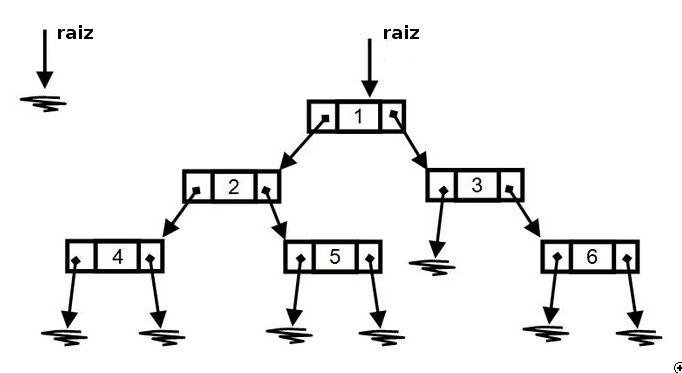
\includegraphics[width=300pt]{imagens/estrutura_arvore.png}
  \label{fig_estrutura_arvore}
\end{figure}
\end{frame}

%%%%%%%%%%%%%%%%%%%%%%%%%%%%%%%%%%%%%%%%%%%%%%%%%%%%%%%%%%%%%%%%%%%%%%%%%%%%%%%%%%%%%%%%%%%%%%%%%%%%%

\begin{frame}[fragile]{Árvore AVL}{Estrutura Árvore}
\begin{algorithm}[H]
\caption{Arvore} 
\label{Arvore}
\Inicio{
 Tipo Nodo* Arvore;
}
\end{algorithm} 
Na linguagem C, a implementação fica conforme o código a seguir:
\begin{lstlisting}[style=CStyle]
typedef nodo* ArvAVL;
\end{lstlisting}  

\end{frame}

%%%%%%%%%%%%%%%%%%%%%%%%%%%%%%%%%%%%%%%%%%%%%%%%%%%%%%%%%%%%%%%%%%%%%%%%%%%%%%%%%%%%%%%%%%%%%%%%%%%%%
\begin{frame}{Árvore AVL}{Inserção}
Agora, vamos implementar dois algoritmos básicos:
\begin{itemize}
 \item {\bf CriaÁrvore}: cria uma árvore vazia.
 \item {\bf ArvoreVazia}: verifica se uma árvore está vazia.
\end{itemize}
\end{frame}
%------------------------------------------------

\section{Algoritmo CriaÁrvore | ÁrvoreVazia}

\begin{frame}{CriaÁrvore | ÁrvoreVazia}{Pseudo-Código}
% \scalebox{0.5}{
\begin{algorithm}[H]
\caption{CriaÁrvore} 
\label{CriaArvoreAVL}
\Saida{Ponteiro $r$ para raiz.}
\Inicio{
    r $\leftarrow$ NULL 
}
\end{algorithm}
% }  
\begin{algorithm}[H]
\caption{ÁrvoreVazia} 
\label{ArvoreVazia}
\Entrada{Ponteiro $r$ para raiz.}
\Saida{V ou F}
\Inicio{
  \Retorna (r = NULL)
  
}
\end{algorithm}
% }  
\end{frame}


%%%%%%%%%%%%%%%%%%%%%%%%%%%%%%%%%%%%%%%%%%%%%%%%%%%%%%%%%%%%%%%%%%%%%%%%%%%%%%%%%%%%%%%%%%%%%%%%%%%%%

\begin{frame}[fragile]{CriaÁrvoreAVL | ÁrvoreVazia}{Código-Fonte}
Na linguagem C, a implementação fica conforme o código a seguir:
\begin{lstlisting}[style=CStyle]
ArvAVL* cria_arvore_avl() {
    ArvAVL* raiz = (ArvAVL*) malloc(sizeof(ArvAVL));
    if(raiz != NULL)
        *raiz = NULL;
    return raiz;   
}

int arvore_vazia(nodo *r) {
    return r == NULL;
}
\end{lstlisting}  
\end{frame}

%%%%%%%%%%%%%%%%%%%%%%%%%%%%%%%%%%%%%%%%%%%%%%%%%%%%%%%%%%%%%%%%%%%%%%%%%%%%%%%%%%%%%%%%%%%%%%%%%%%%%
\section{Altura Nodo | Fator Balanceamento | Maior}
%%%%%%%%%%%%%%%%%%%%%%%%%%%%%%%%%%%%%%%%%%%%%%%%%%%%%%%%%%%%%%%%%%%%%%%%%%%%%%%%%%%%%%%%%%%%%%%%%%%%%

\begin{frame}{Altura Nodo | Fator Balanceamento | Maior}{Introdução}
Agora, vamos implementar dois algoritmos básicos:
\begin{itemize}
 \item {\bf AlturaNodo}: retorna a altura de um nodo.
 \item {\bf FatorBalanceamento}: retorna o fator de balaceamento de um nodo.
 \item {\bf Maior}: retorna compara dois elementos, retornando o maior.
\end{itemize}
\end{frame}

%%%%%%%%%%%%%%%%%%%%%%%%%%%%%%%%%%%%%%%%%%%%%%%%%%%%%%%%%%%%%%%%%%%%%%%%%%%%%%%%%%%%%%%%%%%%%%%%%%%%%

\begin{frame}{Altura Nodo}{Pseudo-Código}
% \scalebox{0.8}{
\begin{algorithm}[H]
\caption{AlturaNodo} 
\label{AlturaNodo}
\Entrada{Ponteiro para o nodo $n$.}
\Saida{Altura do nodo $n$.}
\Inicio{
  \Se {(n = NULL)} {
    \Retorna ( -1  )
  }
  \Senao {
    \Retorna n.altura
  }
}
\end{algorithm}
% }  
\tiny{Adaptado de \cite{Backes2016}}  
\end{frame}

%%%%%%%%%%%%%%%%%%%%%%%%%%%%%%%%%%%%%%%%%%%%%%%%%%%%%%%%%%%%%%%%%%%%%%%%%%%%%%%%%%%%%%%%%%%%%%%%%%%%%

\begin{frame}[fragile]{Altura Nodo}{Código-Fonte}
Na linguagem C, a implementação fica conforme o código a seguir:
\begin{lstlisting}[style=CStyle]
int altura_nodo(nodo* no){
    if(no == NULL)
        return -1;
    else
		return no->altura;
}
\end{lstlisting}  
\end{frame}

%%%%%%%%%%%%%%%%%%%%%%%%%%%%%%%%%%%%%%%%%%%%%%%%%%%%%%%%%%%%%%%%%%%%%%%%%%%%%%%%%%%%%%%%%%%%%%%%%%%%%

\begin{frame}{Fator de Balanceamento}{Pseudo-Código}
\begin{algorithm}[H]
\caption{FatorBalanceamento} 
\label{FatorBalanceamento}
\Entrada{Ponteiro para o nodo $n$.}
\Inicio{
  \Retorna abs(AlturaNodo(n.esq) - AlturaNodo(n.dir))
}
\end{algorithm}
\end{frame}

%%%%%%%%%%%%%%%%%%%%%%%%%%%%%%%%%%%%%%%%%%%%%%%%%%%%%%%%%%%%%%%%%%%%%%%%%%%%%%%%%%%%%%%%%%%%%%%%%%%%%

\begin{frame}[fragile]{Fator de Balanceamento}{Código-Fonte}
Na linguagem C, a implementação fica conforme o código a seguir:
\begin{lstlisting}[style=CStyle]
int fator_balanceamento_nodo(nodo* no){
    return labs(altura_nodo(no->esq) - altura_nodo(no->dir));
}
\end{lstlisting}  
\end{frame}


%%%%%%%%%%%%%%%%%%%%%%%%%%%%%%%%%%%%%%%%%%%%%%%%%%%%%%%%%%%%%%%%%%%%%%%%%%%%%%%%%%%%%%%%%%%%%%%%%%%%%

\begin{frame}[fragile]{Maior}{Código-Fonte}
Na linguagem C, a implementação da função {\bf Maior} fica conforme o código a seguir:
\begin{lstlisting}[style=CStyle]
int maior(int x, int y){
    if(x > y)
        return x;
    else
        return y;
}
\end{lstlisting}  
\end{frame}

%%%%%%%%%%%%%%%%%%%%%%%%%%%%%%%%%%%%%%%%%%%%%%%%%%%%%%%%%%%%%%%%%%%%%%%%%%%%%%%%%%%%%%%%%%%%%%%%%%%%%
\section{Rotações}
%%%%%%%%%%%%%%%%%%%%%%%%%%%%%%%%%%%%%%%%%%%%%%%%%%%%%%%%%%%%%%%%%%%%%%%%%%%%%%%%%%%%%%%%%%%%%%%%%%%%%

\begin{frame}{Rotação LL}{Pseudo-Código}
% \scalebox{0.8}{
\begin{algorithm}[H]
\caption{RotaçãoLL} 
\label{RotacaoLL}
\Entrada{Ponteiro para o nodo desbalanceado $A$.}
\Inicio{
  B $\leftarrow$ A.esq \\
  A.esq $\leftarrow$ B.dir \\
  B.dir $\leftarrow$ A \\
  A.altura $\leftarrow$ maior(AlturaNodo(A.esq), AlturaNodo(A.dir)) + 1 \\
  B.altura $\leftarrow$ maior(AlturaNodo(B.esq), A.altura) + 1 \\
  A $\leftarrow$ B \\
}
\end{algorithm}
% }  
\tiny{Adaptado de \cite{Backes2016}}  
\end{frame}

%%%%%%%%%%%%%%%%%%%%%%%%%%%%%%%%%%%%%%%%%%%%%%%%%%%%%%%%%%%%%%%%%%%%%%%%%%%%%%%%%%%%%%%%%%%%%%%%%%%%%

\begin{frame}[fragile]{Rotação LL}{Código-Fonte}
Na linguagem C, a implementação fica conforme o código a seguir:
\begin{lstlisting}[style=CStyle]
void rotacao_LL(ArvAVL *A){
    nodo *B;
    B = (*A)->esq;
    (*A)->esq = B->dir;
    B->dir = *A;
    (*A)->altura = maior(altura_nodo((*A)->esq),altura_nodo((*A)->dir)) + 1;
    B->altura = maior(altura_nodo(B->esq),(*A)->altura) + 1;
    *A = B;
}
\end{lstlisting}  
\end{frame}

%%%%%%%%%%%%%%%%%%%%%%%%%%%%%%%%%%%%%%%%%%%%%%%%%%%%%%%%%%%%%%%%%%%%%%%%%%%%%%%%%%%%%%%%%%%%%%%%%%%%%

\begin{frame}{Rotação RR}{Pseudo-Código}
% \scalebox{0.8}{
\begin{algorithm}[H]
\caption{RotaçãoRR} 
\label{RotacaoRR}
\Entrada{Ponteiro para o nodo desbalanceado $A$.}
\Inicio{
  B $\leftarrow$ A.dir \\
  A.dir $\leftarrow$ B.esq \\
  B.esq $\leftarrow$ A \\
  A.altura $\leftarrow$ maior(AlturaNodo(A.esq), AlturaNodo(A.dir)) + 1 \\
  B.altura $\leftarrow$ maior(AlturaNodo(B.dir), A.altura) + 1 \\
  A $\leftarrow$ B \\
}
\end{algorithm}
% }  
\tiny{Adaptado de \cite{Backes2016}}  
\end{frame}

%%%%%%%%%%%%%%%%%%%%%%%%%%%%%%%%%%%%%%%%%%%%%%%%%%%%%%%%%%%%%%%%%%%%%%%%%%%%%%%%%%%%%%%%%%%%%%%%%%%%%

\begin{frame}[fragile]{Rotação RR}{Código-Fonte}
Na linguagem C, a implementação fica conforme o código a seguir:
\begin{lstlisting}[style=CStyle]
void rotacao_RR(ArvAVL *A){
    nodo *B;
    B = (*A)->dir;
    (*A)->dir = B->esq;
    B->esq = (*A);
    (*A)->altura = maior(altura_nodo((*A)->esq),altura_nodo((*A)->dir)) + 1;
    B->altura = maior(altura_nodo(B->dir),(*A)->altura) + 1;
    (*A) = B;
}
\end{lstlisting}  
\end{frame}

%%%%%%%%%%%%%%%%%%%%%%%%%%%%%%%%%%%%%%%%%%%%%%%%%%%%%%%%%%%%%%%%%%%%%%%%%%%%%%%%%%%%%%%%%%%%%%%%%%%%%

\begin{frame}{Rotação RL}
% \scalebox{0.8}{
\begin{algorithm}[H]
\caption{RotaçãoRL} 
\label{RotacaoRL}
\Entrada{Ponteiro para a raiz $r$.}
\Inicio{
  RotaçãoLL(r.dir) \\
  RotaçãoRR(r) \\
}
\end{algorithm}
% }  
\tiny{Adaptado de \cite{Backes2016}}  
\end{frame}


%%%%%%%%%%%%%%%%%%%%%%%%%%%%%%%%%%%%%%%%%%%%%%%%%%%%%%%%%%%%%%%%%%%%%%%%%%%%%%%%%%%%%%%%%%%%%%%%%%%%%

\begin{frame}[fragile]{Rotação RL}{Código-Fonte}
Na linguagem C, a implementação fica conforme o código a seguir:
\begin{lstlisting}[style=CStyle]
void rotacao_RL(ArvAVL *A){
    rotacao_LL(&(*A)->dir);
    rotacao_RR(A);
}
\end{lstlisting}  
\end{frame}

%%%%%%%%%%%%%%%%%%%%%%%%%%%%%%%%%%%%%%%%%%%%%%%%%%%%%%%%%%%%%%%%%%%%%%%%%%%%%%%%%%%%%%%%%%%%%%%%%%%%%

\begin{frame}{Rotação LR}
% \scalebox{0.8}{
\begin{algorithm}[H]
\caption{RotaçãoLR} 
\label{RotacaoLR}
\Entrada{Ponteiro para a raiz $r$.}
\Inicio{
  RotaçãoRR(r.esq) \\
  RotaçãoLL(r) \\
}
\end{algorithm}
% }  
\tiny{Adaptado de \cite{Backes2016}}  
\end{frame}

%%%%%%%%%%%%%%%%%%%%%%%%%%%%%%%%%%%%%%%%%%%%%%%%%%%%%%%%%%%%%%%%%%%%%%%%%%%%%%%%%%%%%%%%%%%%%%%%%%%%%

\begin{frame}[fragile]{Rotação LR}{Código-Fonte}
Na linguagem C, a implementação fica conforme o código a seguir:
\begin{lstlisting}[style=CStyle]
void rotacao_LR(ArvAVL *A){
    rotacao_RR(&(*A)->esq);
    rotacao_LL(A);
}
\end{lstlisting}  
\end{frame}


%%%%%%%%%%%%%%%%%%%%%%%%%%%%%%%%%%%%%%%%%%%%%%%%%%%%%%%%%%%%%%%%%%%%%%%%%%%%%%%%%%%%%%%%%%%%%%%%%%%%%
\section{Inserir}
%%%%%%%%%%%%%%%%%%%%%%%%%%%%%%%%%%%%%%%%%%%%%%%%%%%%%%%%%%%%%%%%%%%%%%%%%%%%%%%%%%%%%%%%%%%%%%%%%%%%%

\begin{frame}{Inserir}{Pseudocódigo}
% \scalebox{0.5}{
\begin{algorithm}[H]
\caption{InserirAVL} 
\label{InserirAVL}
\Entrada{Ponteiro para a raiz $r$, item $x$.}
\Saida{V ou F}
\Inicio{
  \Se {( r = NULL)} {
    novo $\leftarrow$ ALOCA\_NODO() \\
    novo.item $\leftarrow$ x \\
    novo.altura $\leftarrow$ 0\\
    novo.esq $\leftarrow$ NULL \\
    novo.dir $\leftarrow$ NULL \\
    r $\leftarrow$ novo \\
    \Retorna Verdadeiro
   }
}
\rememberlines
\end{algorithm}
% }  
\end{frame}

%%%%%%%%%%%%%%%%%%%%%%%%%%%%%%%%%%%%%%%%%%%%%%%%%%%%%%%%%%%%%%%%%%%%%%%%%%%%%%%%%%%%%%%%%%%%%%%%%%%%%

\begin{frame}{Inserir}{Pseudocódigo InserirAVL}
\scalebox{0.6}{
\begin{algorithm}[H]
\resumenumbering
\caption{InserirAVL (continuação)} 
\label{InserirAVL2}
% \Entrada{Ponteiro para a raiz $r$, item $x$.}
% \Saida{V ou F}
\Inicio{
   atual $\leftarrow$ r \\
   \Se {(x $<$ atual.item)} {
     \Se {(InserirAVL(atual.esq, x))} { \label{inserir_avl_condicao1}
       \Se{(FatorBalanceamento(atual) $\geq 2$)} {
	  \Se {(x $<$ r.esq.item)} {
	    RotacaoLL(r) \\
	  }
	  \Senao {
	    RotacaoLR(r)\\
	  }
	}
      }
    }
    \Senao {
      \Se {(x $>$ atual.item)} {
	\Se{(InserirAVL(atual.dir, x))} { \label{inserir_avl_condicao2}
	  \Se{(FatorBalanceamento(atual) $\geq 2$)} {
	    \Se{(r.dir.item $<$ x)} {
	      RotacaoRR(r)\\
	    }
	    \Senao {
	      RotacaoRL(r)\\
	    }
	  }
	}
      }
      \Senao {
	\Retorna Falso
      }
    }
    atual.alt $\leftarrow$ maior(AlturaNodo(atual.esq),AlturaNodo(atual.dir)) + 1 \label{inserir_avl_atualiza_altura}\\
    \Retorna Verdadeiro    
}
\end{algorithm}
}  
\tiny{Adaptado de \cite{Backes2016}}  
\end{frame}

%%%%%%%%%%%%%%%%%%%%%%%%%%%%%%%%%%%%%%%%%%%%%%%%%%%%%%%%%%%%%%%%%%%%%%%%%%%%%%%%%%%%%%%%%%%%%%%%%%%%%

\begin{frame}[fragile]{Inserir}{Código-Fonte - Parte 1}
Na linguagem C, a implementação fica conforme o código a seguir:
\begin{lstlisting}[style=CStyle]
int insere_ArvAVL(ArvAVL *raiz, int valor){
    int res;
    if (*raiz == NULL){
        nodo *novo;
        novo = (nodo*)malloc(sizeof(nodo));
        if(novo == NULL)
            return 0;

        novo->item = valor;
        novo->altura = 0;
        novo->esq = NULL;
        novo->dir = NULL;
        *raiz = novo;
        return 1;
    }
    nodo *atual = *raiz;
    /** Continua no proximo slide **/   
\end{lstlisting}  
\end{frame}

%%%%%%%%%%%%%%%%%%%%%%%%%%%%%%%%%%%%%%%%%%%%%%%%%%%%%%%%%%%%%%%%%%%%%%%%%%%%%%%%%%%%%%%%%%%%%%%%%%%%%

\begin{frame}[fragile]{Inserir}{Código-Fonte - Parte 2}
\begin{lstlisting}[style=CStyle,firstnumber=16]
    nodo *atual = *raiz;
    /** Continuacao do slide anterior **/
    if (valor < atual->item){
        if ((res = insere_ArvAVL(&(atual->esq), valor)) == 1){
            if (fator_balanceamento_nodo(atual) >= 2){
                if (valor < (*raiz)->esq->item ){
                    rotacao_LL(raiz);
                } else {
                    rotacao_LR(raiz);
                }
            }
        }
    } else {
        if (valor > atual->item){
        /** Continua no proximo slide **/        
\end{lstlisting}  
\end{frame}

%%%%%%%%%%%%%%%%%%%%%%%%%%%%%%%%%%%%%%%%%%%%%%%%%%%%%%%%%%%%%%%%%%%%%%%%%%%%%%%%%%%%%%%%%%%%%%%%%%%%%

\begin{frame}[fragile]{Inserção}{Código-Fonte - Parte 3}
\begin{lstlisting}[style=CStyle,firstnumber=29]
        if (valor > atual->item){
            /** Continuacao do slide anterior **/        
            if ((res = insere_ArvAVL(&(atual->dir), valor)) == 1){
                if (fator_balanceamento_nodo(atual) >= 2){
                    if((*raiz)->dir->item < valor) {
                        rotacao_RR(raiz);
                    } else {
                        rotacao_RL(raiz);
                    }
                }
            }
        } else {
            printf("Valor duplicado!!\n");
            return 0;
        }
    }
    atual->altura=maior(altura_nodo(atual->esq),altura_nodo(atual->dir))+1;
    return res;
}
\end{lstlisting}  
\end{frame}

%%%%%%%%%%%%%%%%%%%%%%%%%%%%%%%%%%%%%%%%%%%%%%%%%%%%%%%%%%%%%%%%%%%%%%%%%%%%%%%%%%%%%%%%%%%%%%%%%%%%%
\section{Remover}
%%%%%%%%%%%%%%%%%%%%%%%%%%%%%%%%%%%%%%%%%%%%%%%%%%%%%%%%%%%%%%%%%%%%%%%%%%%%%%%%%%%%%%%%%%%%%%%%%%%%%

\begin{frame}{Remover}{Algoritmo ProcuraMaior}
% \scalebox{0.8}{
\begin{algorithm}[H]
\caption{ProcuraMaior} 
\label{ProcuraMaior}
\Entrada{Ponteiro para o nodo {\bf atual}.}
\Saida{Ponteiro para o maior valor a partir do nodo {\bf atual}.}
\Inicio{
    n1 $\leftarrow$ atual\\
    n2 $\leftarrow$ atual.dir\\
    \Enqto {(n2$\neq$ NULL)} {
      n1 $\leftarrow$ n2\\
      n2 $\leftarrow$ n2.dir\\
    }
    \Retorna n1
}
\end{algorithm}
% }  
\tiny{Adaptado de \cite{Backes2016}}  
\end{frame}

%%%%%%%%%%%%%%%%%%%%%%%%%%%%%%%%%%%%%%%%%%%%%%%%%%%%%%%%%%%%%%%%%%%%%%%%%%%%%%%%%%%%%%%%%%%%%%%%%%%%%

\begin{frame}{Remover}{Algoritmo RemoverAVL}
\scalebox{0.6}{
\begin{algorithm}[H]
\caption{RemoverAVL} 
\label{RemoverAVL}
\Entrada{Ponteiro para a raiz $r$, item $x$.}
\Saida{V ou F}
\Inicio{
  \Se{(r = NULL)} { \label{remover_avl_arvore_vazia}
    \Retorna Falso
  }
  \Se{(x $<$ r.item)} { \label{remover_avl_x_menor}
    \Se{(RemoverAVL(r.esq, x))} { \label{remover_avl_teste_recursivo1}
      \Se{(FatorBalanceamento(r) $\geq$ 2)} { \label{remover_avl_teste_balanceamento_inicio1}
			\Se {(AlturaNodo(r.dir.esq) $\leq$ AlturaNodo(r.dir.dir))} {
	  			RotacaoRR(r) \\
			}
			\Senao {
	  			RotacaoRL(r) \\
			}
      } \label{remover_avl_teste_balanceamento_fim1}
    }
  }
  \Se{(x $>$ r.item )} {  \label{remover_avl_x_maior}
    \Se{(RemoverAVL(r.dir, x))} { \label{remover_avl_teste_recursivo2}
      \Se{(FatorBalanceamento(r) $\geq$ 2)} { \label{remover_avl_teste_balanceamento_inicio2}
			\Se {(AlturaNodo(r.esq.dir) $\leq$ AlturaNodo(r.esq.esq))} {
				  RotacaoLL(r) \\
			}
			\Senao {
				  RotacaoLR(r) \\
			}
      	} \label{remover_avl_teste_balanceamento_fim2}	
    } 
  }  
  \rememberlines
}
\end{algorithm}
}  
\tiny{Adaptado de \cite{Backes2016}}  
\end{frame}

%%%%%%%%%%%%%%%%%%%%%%%%%%%%%%%%%%%%%%%%%%%%%%%%%%%%%%%%%%%%%%%%%%%%%%%%%%%%%%%%%%%%%%%%%%%%%%%%%%%%%

\begin{frame}{Remover}{Algoritmo RemoverAVL}
\scalebox{0.5}{
\begin{algorithm}[H]
\caption{RemoverAVL (Continuação)} 
\label{RemoverAVL2}
\resumenumbering
\Inicio{
  \Se {(r.item = x)} { \label{remover_avl_remocao_inicio}
    \Se{(r.esq = NULL) ou (r.dir = NULL)} { \label{remover_avl_nodo_folha}
      removerNodo $\leftarrow$ r \label{remover_avl_nodo_auxiliar} \\ 
      \Se {(r.esq $\neq$ NULL)} { \label{remover_avl_nodo_folha_atualiza_filho_inicio}
			r $\leftarrow$ r.esq \\
      }
      \Senao { \label{remover_avl_nodo_folha_raiz_null_inicio}
			r $\leftarrow$ r.dir \label{remover_avl_nodo_folha_atualiza_raiz_null_fim}\\
      } \label{remover_avl_nodo_folha_atualiza_filho_fim}
      DESALOCA\_NODO(removerNodo) \label{remover_avl_nodo_folha_libera_memoria} \\      
    } 
    \Senao { \label{remover_avl_nodo_dois_filhos_inicio}
      	antecessor $\leftarrow$ ProcuraMaior(r.dir) \label{remover_avl_busca_antecessor} \\
      	r.item $\leftrightarrow$ antecessor.item \CommentSty{// Troca os valores.} \label{remover_avl_troca_raiz_antecessor} \\
      	RemoverAVL(r.dir, antecessor.item) \label{remover_avl_remover_antecessor} \\
      	\Se {(FatorBalanceamento(r) $\geq$ 2)} { \label{remover_avl_verifica_balanceamento}
			\Se{AlturaNodo(r.esq.dir) $\leq$ AlturaNodo(r.esq.esq)} { \label{remover_avl_verifica_altura}
	  			RotaçãoLL(r) \label{remover_avl_rotacao_simples} \\
		}
		\Senao {
	  		RotaçãoLR(r) \label{remover_avl_rotacao_dupla} \\
		}
      }
      \Se{(r $\neq$ NULL)} {
			r.altura $\leftarrow$ maior(AlturaNodo(r.esq), AlturaNodo(r.dir)) + 1 \\
      }
      \Retorna Verdadeiro
    } \label{remover_avl_nodo_dois_filhos_fim}
    r.altura $\leftarrow$ maior(AlturaNodo(r.esq), AlturaNodo(r.dir)) + 1 \\
    \Retorna Verdadeiro \label{remover_avl_retorna_verdadeiro}
  }
}  \label{remover_avl_remocao_fim}
\end{algorithm}
}  
\tiny{Adaptado de \cite{Backes2016}}  
\end{frame}

%%%%%%%%%%%%%%%%%%%%%%%%%%%%%%%%%%%%%%%%%%%%%%%%%%%%%%%%%%%%%%%%%%%%%%%%%%%%%%%%%%%%%%%%%%%%%%%%%%%%%

\begin{frame}[fragile]{Remover}{Código-Fonte - Parte 1}
Na linguagem C, a implementação fica conforme o código a seguir:
\begin{lstlisting}[style=CStyle,basicstyle=\tiny]
int remove_ArvAVL(ArvAVL *raiz, int valor){
	if(*raiz == NULL){
	    printf("Valor nao existe!!\n");
	    return 0;
	}
	int res;
	if(valor < (*raiz)->item){
	    if((res = remove_ArvAVL(&(*raiz)->esq,valor)) == 1){
            if(fator_balanceamento_nodo(*raiz) >= 2){
                if(altura_nodo((*raiz)->dir->esq) <= altura_nodo((*raiz)->dir->dir))
                    rotacao_RR(raiz);
                else
                    rotacao_RL(raiz);
            }
	    }
	}
    /** Continua no proximo slide **/   
\end{lstlisting}  
\end{frame}

%%%%%%%%%%%%%%%%%%%%%%%%%%%%%%%%%%%%%%%%%%%%%%%%%%%%%%%%%%%%%%%%%%%%%%%%%%%%%%%%%%%%%%%%%%%%%%%%%%%%%

\begin{frame}[fragile]{Remover}{Código-Fonte - Parte 2}
\begin{lstlisting}[style=CStyle,basicstyle=\tiny,firstnumber=17]
    /** Continuacao do slide anterior **/    
	if((*raiz)->item < valor){
	    if((res = remove_ArvAVL(&(*raiz)->dir, valor)) == 1){
            if(fator_balanceamento_nodo(*raiz) >= 2){
                if(altura_nodo((*raiz)->esq->dir) <= altura_nodo((*raiz)->esq->esq) )
                    rotacao_LL(raiz);
                else
                    rotacao_LR(raiz);
            }
	    }
	}
	if((*raiz)->item == valor){
	    if(((*raiz)->esq == NULL || (*raiz)->dir == NULL)){
            nodo *oldNode = (*raiz);
            if((*raiz)->esq != NULL)
                *raiz = (*raiz)->esq;
            else
                *raiz = (*raiz)->dir;
            free(oldNode);
        } else { 
            /** Continua no proximo slide **/   
\end{lstlisting}  
\end{frame}

%%%%%%%%%%%%%%%%%%%%%%%%%%%%%%%%%%%%%%%%%%%%%%%%%%%%%%%%%%%%%%%%%%%%%%%%%%%%%%%%%%%%%%%%%%%%%%%%%%%%%

\begin{frame}[fragile]{Remover}{Código-Fonte - Parte 3}
\begin{lstlisting}[style=CStyle,basicstyle=\tiny,firstnumber=36]
        } else { 
            /** Continuacao do slide anterior **/  		
            nodo* temp = procura_menor((*raiz)->dir);
            (*raiz)->item = temp->item;
            remove_ArvAVL(&(*raiz)->dir, (*raiz)->item);
            if(fator_balanceamento_nodo(*raiz) >= 2){
                if(altura_nodo((*raiz)->esq->dir) <= altura_nodo((*raiz)->esq->esq))
                    rotacao_LL(raiz);
                else
                    rotacao_LR(raiz);
            }
        }
        if (*raiz != NULL)
            (*raiz)->altura = maior(altura_nodo((*raiz)->esq), altura_nodo((*raiz)->dir)) + 1;
        return 1;
    }
    (*raiz)->altura = maior(altura_nodo((*raiz)->esq), altura_nodo((*raiz)->dir)) + 1;
    return res;
}
\end{lstlisting}  
\end{frame}

%%%%%%%%%%%%%%%%%%%%%%%%%%%%%%%%%%%%%%%%%%%%%%%%%%%%%%%%%%%%%%%%%%%%%%%%%%%%%%%%%%%%%%%%%%%%%%%%%%%%%

%\begin{frame}
%\Huge{\centerline{Dúvidas?}}
%
%\begin{figure}[!h]
%  \centering
%  
\includegraphics[width=100pt]{imagens/duvidas.jpg}
%  \label{fig_fim}
%\end{figure}
%\end{frame}

%%%%%%%%%%%%%%%%%%%%%%%%%%%%%%%%%%%%%%%%%%%%%%%%%%%%%%%%%%%%%%%%%%%%%%%%%%%%%%%%%%%%%%%%%%%%%%%%%%%%%
\section{Função Main}
%%%%%%%%%%%%%%%%%%%%%%%%%%%%%%%%%%%%%%%%%%%%%%%%%%%%%%%%%%%%%%%%%%%%%%%%%%%%%%%%%%%%%%%%%%%%%%%%%%%%%

\begin{frame}{Função Main}{Introdução}
Por fim, falta apenas criar uma {\bf função Main} para manipular nossa estrutura de dados Árvore AVL.
\end{frame}

%%%%%%%%%%%%%%%%%%%%%%%%%%%%%%%%%%%%%%%%%%%%%%%%%%%%%%%%%%%%%%%%%%%%%%%%%%%%%%%%%%%%%%%%%%%%%%%%%%%%%

\begin{frame}[fragile]{Função Main}{Código-Fonte Apagar Árvore}
\begin{lstlisting}[style=CStyle,basicstyle=\tiny]
int main() {
    int rand_max = 10; int vaux = 0;
    srand(42);
    ArvAVL *arvore_avl;
    arvore_avl = cria_arvore_avl();
    for (int i = 0; i < 20; i++) {
        insere_ArvAVL(arvore_avl, rand() % rand_max);
    }
    printf("\nPercurso Pre-Ordem\n");
    pre_ordem(arvore_avl);
    printf("\nPercurso Em-Ordem\n");
    em_ordem(arvore_avl);
    printf("\nPercurso Pos-Ordem\n");
    pos_ordem(arvore_avl);
    vaux = rand() % rand_max;
    printf("\nRemover valor %d\n", vaux);
    remove_ArvAVL(arvore_avl, vaux);

    apagar_ArvAVL(arvore_avl);
    return 0;
}
\end{lstlisting}  
\end{frame}


%%%%%%%%%%%%%%%%%%%%%%%%%%%%%%%%%%%%%%%%%%%%%%%%%%%%%%%%%%%%%%%%%%%%%%%%%%%%%%%%%%%%%%%%%%%%%%%%%%%%%

\begin{frame}{Referências}{Bibliografia Básica}
\begin{itemize}
\item Bibliografia Básica
\bibliographystyle{abnt-alf}
\bibliography{referencias}
\item Material Complementar
\begin{itemize}
\item \href{https://programacaodescomplicada.wordpress.com/complementar/}{Código-fonte e listas de exercícios - Material disponível on-line}
\end{itemize}
\item Vídeo-aulas
\begin{itemize}
\item \href{https://www.youtube.com/watch?v=Au-6c55J90c&index=78&list=PL8iN9FQ7_jt6H5m4Gm0H89sybzR9yaaka}{Canal do youtube do prof. André Backes.}
\item \href{https://www.youtube.com/watch?v=YkF76cOgtMQ&t=92s}{Vídeo-aula: Estrutura de dados - Univesp}
\end{itemize}
\item Animação
\begin{itemize}
\item \href{https://www.cs.usfca.edu/~galles/visualization/AVLtree.html}{Árvore AVL - USFCA}
\item \href{http://www.cs.armstrong.edu/liang/animation/web/AVLTree.html}{Árvore AVL - CS - Armstrong}
\end{itemize}
\end{itemize}
\end{frame}

%%%%%%%%%%%%%%%%%%%%%%%%%%%%%%%%%%%%%%%%%%%%%%%%%%%%%%%%%%%%%%%%%%%%%%%%%%%%%%%%%%%%%%%%%%%%%%%%%%%%%%%%%%
\begin{frame}[plain]
  \titlepage
\end{frame}

\end{document}
